% !TeX root = ../main.tex

\chapter{相关技术简介}
在前一章对本课题的选题背景以及研究意义进行了详细地阐述,也介绍了本论文主要解决的问题。本章首先会介绍对象存储的相关知识,并辨析对象存储与文件存储和块存储的区别,然后介绍了一些典型的分布式存储系统,这些系统的实现对本系统的实现有重要指导作用,同时本章也会对系统实现中需要用到的技术进行介绍与分析,并对这些技术的优势进行分析。
\section{对象存储}%2.1
\subsection{对象存储系统体系结构}%2.1.1
对象存储是一种以对象为单位的存储方式,通常用来存储非结构化数据,用户的每一个数据都可以被抽象为对象,每一个对象都有一个唯一的标识符,系统根据标识符来对对象进行管理,对象的元数据和实际数据分开存放。对象存储不使用目录树来管理文件,而是用桶(bucket)来进行管理,任何对象都需要放置在一个桶中,可以对桶设置相关的属性来批量管理对象。对象存储系统一般会提供RESTful接口进行数据的访问,用户只需提供对象的标识符即可访问系统中的数据,扁平化的结构使用非常方便,特别适合图片视频等非结构化数据的存放。对象存储系统的典型架构如图2.1所示。
\begin{figure}
    \centering
    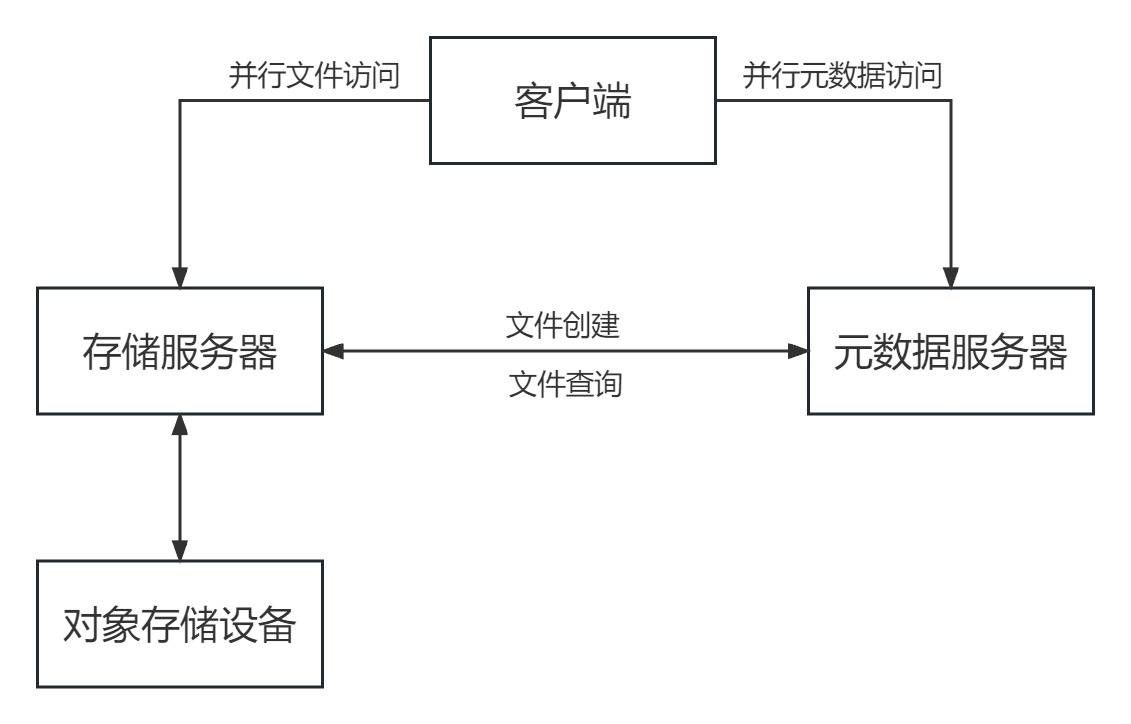
\includegraphics[width=0.8\textwidth]{对象存储架构图.jpg}
    \caption{对象存储架构图}
\end{figure}

用户使用客户端来访问对象存储系统,用户可以通过和元数据服务器交互获得文件的相关信息,也可以对桶进行修改权限等操作,用户访问对象时,需要先从元数据服务器中获取文件的相关元数据,然后将这些元数据传递给存储服务器,存储服务器根据这些信息可以知道文件的存放位置,将数据读取后进行整合,返回给客户端,最终将用户所需的文件返回给用户。存储服务器和元数据服务器也可以互相进行访问,当需要创建文件时,存储服务器需要将文件的信息传递给元数据服务器,元数据服务器会将新文件的信息进行记录,以便下次进行访问时获取到该文件的存储位置。

\subsection{对象存储的特点和优势}%2.1.2
根据存储内容不同,分布式存储可以分为文件存储、块存储和对象存储。这三类存储最大的区别是访问时提供的接口不同。文件存储适配POSIX存储语义,按照人们熟知的文件系统的架构来分配文件的路径,向用户提供文件访问的接口,功能最为完备。块存储提供的接口以数据块为单位,对客户端暴露出来的是“盘”或者“逻辑盘”,数据访问的语义比较简单,主要是对“盘”按照地址偏移访问数据。对象存储是一种将数据作为对象进行存储的方式,没有采用文件存储中的树状目录结构,而是采用键值对的方式,用一个文件名来定位文件,名字空间相对扁平。除了提供的访问接口不同之外,这三类存储所适用的数据类型和提供的操作也不同。文件存储提供了丰富的访问操作,可以随时修改文件的内容,可以利用目录和硬链接构建数据之间的“图”包含关系。对象存储不支持修改对象数据,不能随机访问,平坦的名字空间要借助于其他的数据管理方式才能构建简单的数据集合和数据关系。块存储每个逻辑块的大小是固定的,易于管理和维护,但扩展性较差,无法根据实际需求进行调整,不适合直接存储用户所需保存的数据。

存储的单位不同,系统的优势和缺陷就不一样,以文件作为存储单位,可以利用通用的接口使数据更方便地进行共享,便于人们对文件进行管理和操作,但系统设计复杂\cite{20},当文件数量增加时,系统需要用很多额外空间保存文件的树状目录结构,对这些元数据的管理导致系统存储效率下降也会影响文件的读写性能,同时元数据与文件内容过于耦合,二者依赖过于紧密,不利于节点的扩展;以块作为存储单位,可以提供共享数据的快速访问,但缺少元数据的维护和相关的访问授权,直接的访问方式会存在安全问题\cite{21}。

对象存储兼具文件存储和块存储的优点,能够将文件进行共享的同时还具有高效的文件读写速率\cite{22}。一方面对象存储没有采用文件存储中的树状目录结构,避免了目录数据在传输中的效率低的问题,扁平化数据内容存储提高了数据的读写效率,另一方面对象存储提供了更适合用户使用的接口,不再以块为单位,非常适合非结构化数据的读取和写入。

在功能上,对象存储结合了NAS\cite{23}(Network Attached Storage)和SAN\cite{24} (Storage Area Network)的特点,使对象存储系统拥有优秀的跨平台性能\cite{25},不同的平台系统可以通过对象存储系统进行高效的数据交流。除此之外,由于对象存储系统的元数据和实际数据分离,且没有传统的层次结构的限制,因此对象存储有较好的易用性,数据的读写非常方便,只需给出一个ID就可以定位文件,甚至可以在浏览器中完成基本的数据存储操作,无需特别的软件来支撑。另外,对象存储非常灵活,当数据量增大时,可以通过动态地添加存储设备来实现扩容,理论上可以实现无限扩容,这使得对象存储成为组建PB级存储系统的重要技术。

\section{典型分布式存储系统}%2.2
\subsection{GFS}%2.2.1
谷歌公司的搜索业务是谷歌的核心业务,它们的搜索引擎每天都会产生大量的数据,谷歌公司设计GFS的目的是为了来更好地存储这些数据,这项工程由 “BigFile”项目发展而来。GFS是面向大文件开发的、满足大规模数据型应用的、基于Linux的专有分布式存储系统,高并发环境下它在读多写少时可以发挥更好的性能。GFS允许用户进行横向扩展,利用网络将廉价存储设备聚集,减少用户购买高性能存储设备的成本,同时能够将文件进行一定的冗余处理,可以提供可靠的容灾服务。为了保证系统的性能,GFS采用了弱一致性,使系统响应更加迅速,操作更便捷。

\begin{figure}
    \centering
    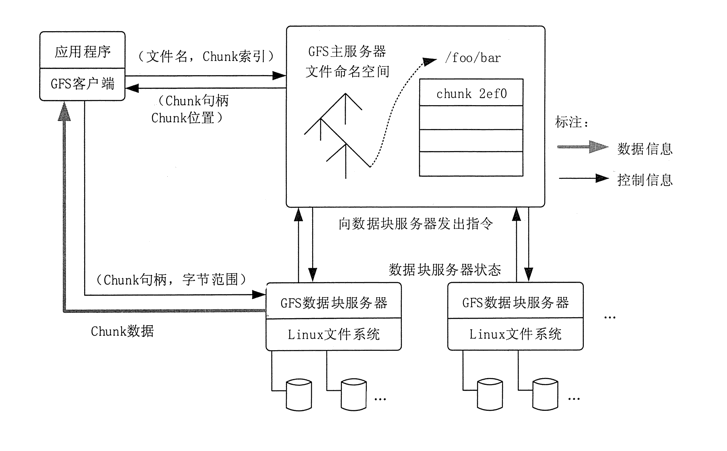
\includegraphics[width=0.9\textwidth]{GFS架构图.png}
    \caption{GFS架构图}
\end{figure}
GFS的设计架构深远地影响了分布式存储系统,因此有必要详细介绍GFS的相关设计原理。GFS的架构如图2.2所示。GFS集群包含了大量节点,这些节点可以分为Master节点和Chunk Server节点,GFS将数据切分成一个个chunk,每个chunk通常为64MB,为了保证数据的可靠,每一个chunk在集群中都有3个以上的副本\cite{26}。Master节点主要负责存储系统的元数据,这些元数据主要包括记录文件存放的物理位置、数据块的冗余信息和当前数据块的访问状态等,Master可以通过Chunk Server发送的心跳来得知这些信息。

GFS为了维护数据的一致性,提出了“租约”的概念,它类似于分布式锁,某个进程只有在租约内才能访问数据块,其他进程在这段租约存在的时候,对数据块的访问将会被限制。数据块被更新后,这个数据块所在的Chunk Server会成为主数据服务器,它会将更改的内容同步到其他Chunk Server上,当其他Chunk Server发送确认后才会将数据持久化,保证了系统数据操作的一致性。


\subsection{Haystack}%2.2.2
在此之后,越来越多的公司为了更好地扩展业务,开始开发属于自己的分布式存储系统。Facebook是一个社交网络服务网站,它为用户保存了海量的照片, Facebook使用CDN来缓存热点图片,但是对于社交网络而言,有大量的请求都不是热点,这些请求被称为长尾请求,而缓存资源比较昂贵,缓存所有的图片是不可能的。为了解决社交网络中海量小文件且请求具有长尾特性的服务能力问题,Facebook开发了一款分布式对象存储系统Haystack。Haystack解决的最重要的问题之一是减少了读取文件时元数据的IO开销,传统文件系统中元数据冗杂且存在磁盘上,导致访问一个文件就要先去磁盘上查找元数据,然后才能知道文件的存放位置,根据得到的置再去找文件,这样的模式在海量小文件查询的场景下成为了瓶颈。图片文件的特点是写一次,读多次,从不修改,很少删除,这些特点和日志文件类似,而日志文件的处理方式是写进一个大文件,因此Haystack的思路是将很多张图片存在同一个文件里面,将小文件变成大文件来进行储存。Haystack包含了三个核心组成部分:Haystack Store,Haystack Directory和Haystack Cache。Directory负责维护逻辑存储和物理存储之间的映射关系,Cache是系统内部的缓存,用于缓存最热的那部分文件。Store内有两种文件,一种是索引文件,它保存了图片在数据文件的具体位置;另一种是数据文件,它保存了一个个Needle,每个Needle保存了图片的实际数据和元数据,正是由于这种文件的存在,大量小文件可以保存在一个大文件中。在Store内可以使用多副本来保证数据的可靠性,一个逻辑文件可以对应多个物理文件,分布在不同的Store上。

\subsection{Ceph}%2.2.2
Ceph\cite{27}利用自身优秀的架构设计,为用户提供了灵活的文件读写接口。Ceph最早出现于Sega博士的博士论文中\cite{28},在这篇论文中介绍了Ceph的核心概念和关键算法。Ceph的架构图如图2.3所示,从下到上可以被分为四个层次。

\begin{figure}
    \centering
    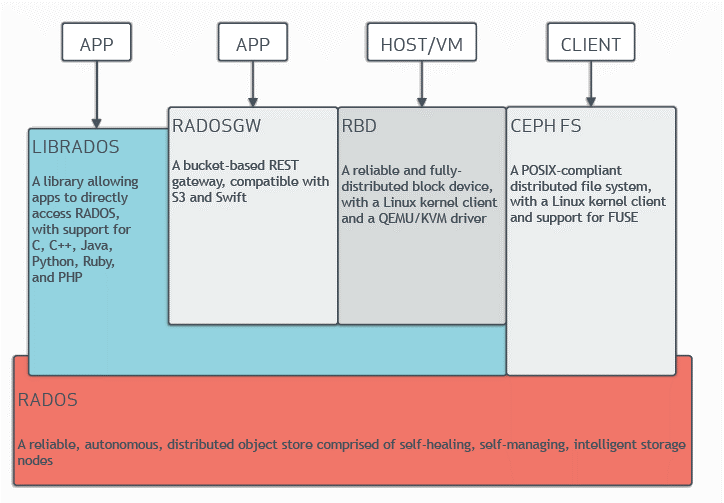
\includegraphics[width=0.7\textwidth]{ceph架构图.png}
    \caption{Ceph架构图}
\end{figure}

1. 基础存储系统RADOS\cite{29,30}

RADOS(Reliable Autonomic Distributed Object Store) 是Ceph的实现基础,它提供了高度可靠和自动管理的对象存储功能,为 Ceph 提供了强大的分布式存储能力。通过RADOS,Ceph可以支持多种不同的数据访问接口,如对象存储、块存储和文件系统接口,使得Ceph成为一个全面且灵活的分布式存储解决方案。在Ceph中,所有数据都以对象的形式在RADOS中进行存储,可以有效保证数据的一致性和可靠性。

在RADOS中,由OSD(Object Store Device)负责数据的存储,RADOS的设计理念是将数据分布在整个Ceph存储集群的多个OSD上。这使得存储集群可以水平扩展,支持海量数据的处理,并具备高性能和负载均衡能力。

RADOS使用CRUSH\cite{31}(Controlled Repplication Under Scalable Hashing)算法进行寻址和负载均衡,当存储集群的节点发生变化或存储容量发生变化时,RADOS会自动调整数据的分布,确保每个OSD上存储的数据量相对均衡。

2. 基础库LIBRADOS

LIBRADOS是Ceph分布式存储系统的用户空间库,它允许应用程序直接与 Ceph 存储集群进行交互。通过 LIBRADOS,开发人员可以利用Ceph存储集群的强大功能,包括对象存储、数据复制、快照、数据恢复等,从而实现高性能和可靠的分布式存储操作。

3. 上层接口RADOSGW、RBD和Ceph FS

为了使用户更方便地对文件进行操作,Ceph为客户端提供了抽象层次更高的接口,它们也是系统的最高层接口,全部基于LIBRADOS层开发\cite{32}。

RADOSGW(Rados Gate Way)提供对象存储服务,是⼀套基于RESTful协议的网关,支持对象存储,兼容S3协议。

RBD(Rados Block Device)提供块存储设备接口,它允许用户创建和管理分布式块设备,并以块存储的方式将这些设备连接到虚拟机、物理服务器或其他应用程序中。RBD为虚拟化环境和需要高性能块存储的应用程序提供了灵活且高效的存储解决方案。

Ceph FS是Ceph提供的一个分布式文件系统,它允许用户在多个节点之间共享文件,并通过标准的POSIX文件系统接口进行访问。Ceph FS 提供了高度可靠和高性能的文件存储解决方案,适用于各种文件共享和存储需求。

4. 用户实例

用户根据自己的需求灵活地调用不同的接口,将文件存储到Ceph中。

\subsection{MinIO}%2.2.3
近些年来,MinIO成为了国外对象存储系统的代表性工作,由于其开源的特性,深受开发者和企业欢迎。MinIO是一款专门为对象存储设计的分布式存储系统,单对象最大可达5TB\cite{33},非常适合存储视频、图片等非结构化数据,这些数据的存储在大数据分析和人工智能等领域有广泛的需求。MinIO 主要采用Go语言实现,借助Go语言中协程的实现,系统无需切换到内核态运行,客户端通过访问存储服务器暴露的HTTP接口进行通信。由于MinIO只实现对象存储接口,所以设计非常简洁,它的核心服务器代码大约只有40MB,用极其轻量的代码实现对象存储所需要的全部功能,例如能够保证加密的数据安全,提供单点登录等。这样设计的好处是,MinIO不仅在性能上强劲高效,而且它具有弹性伸缩的能力,能够更简单地实现动态扩展,提供灵活高效的对象存储服务。

在纠删码的应用上,MinIO为了提升性能,使用汇编代码来编写纠删码应用的相关逻辑。MinIO支持自主配置冗余级别,用户可以自主配置冗余级别来实现不同的数据保护模式,即使丢失了一部分数据,仍然可以从冗余数据中重建数据。此外,MinIO的恢复是基于对象的,一次操作可以修复整个对象的数据。

在一个集群内,MinIO 将自动创建多个纠删组,数据将会按照一定的算法分布在这些纠删组中。若某个纠删组中的数据出现异常或丢失,在一定的故障域内,可以用纠删码算法对异常的数据进行恢复。MinIO集群的架构如图2.4所示,图中所示的集群由四个节点组成,这四个节点会自动建立纠删组,数据将存放到纠删组中,计算对应的纠删码来保护数据,数据的分布则会依据MinIO的分布式算法来决定。

\begin{figure}
    \centering
    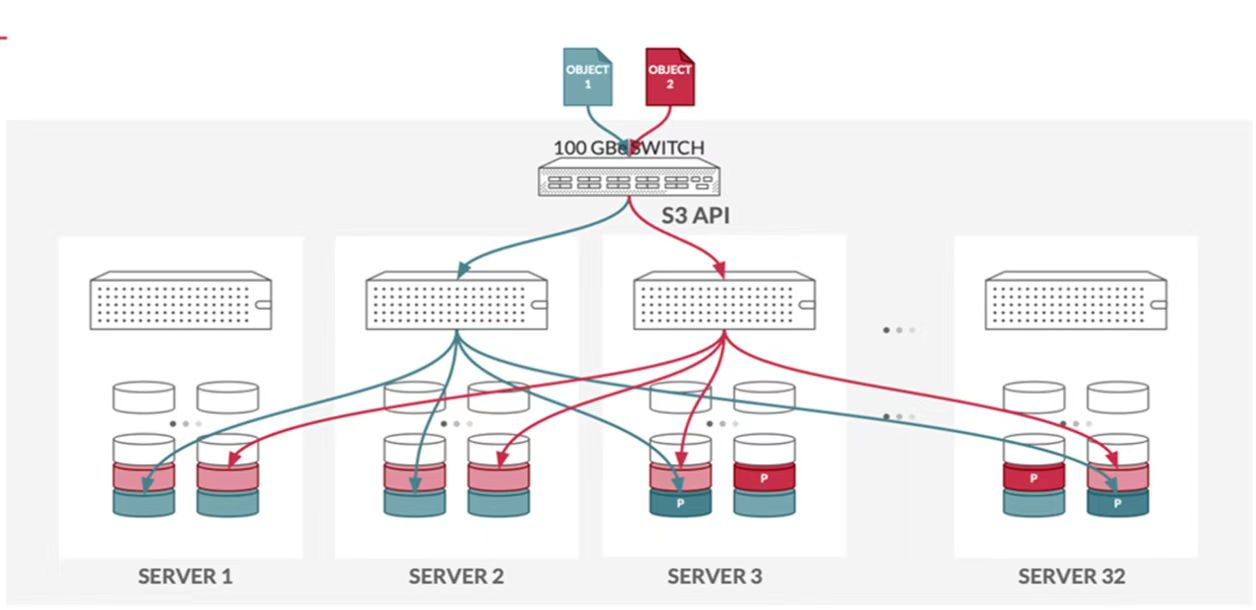
\includegraphics[width=0.9\textwidth]{MinIO架构图.png}
    \caption{MinIO架构图}
\end{figure}

\subsection{NOS}%2.2.4
网易对象存储服务NOS(Netease Object Storage)是网易数帆提供的高可用、高可靠、高性能的云端存储服务。它支持RESTful API接口,主要目标是为用户一站式解决非结构化数据管理问题。NOS支撑大规模的数据量和访问量,利用兼容了S3接口的HTTP协议存储各种文件,对图片文件和视频文件能进行常用的处理(格式转换、加水印、缩略、编解码、截帧等),并支持对不同冷热程度的数据进行分级存储。NOS也支持通过CDN进行访问加速(包括上传加速、Web加速、下载加速等),对跨运营商和全球用户非常友好。

早期的NOS在数据保护方式上采用了三副本的冗余策略,这使得存储成本随着数据规模的不断扩大而快速上涨,因此近几年来NOS开始实践纠删码的数据保护策略,希望以此来降低存储成本。EC策略虽然可以节省空间成本,但是在性能方面与多副本有较大差距,因此NOS采用了分层存储的设计,如图2.5所示。用户写入文件时,具体流程为:用户业务数据先写入副本池,保障其上传性能,当数据在达到某些预设条件(如一段时间无访问等)后,通过LifeCycle程序自动转入EC池,当数据再次被读取时,由EC池提供服务,而且不再转回副本池。

\begin{figure}
    \centering
    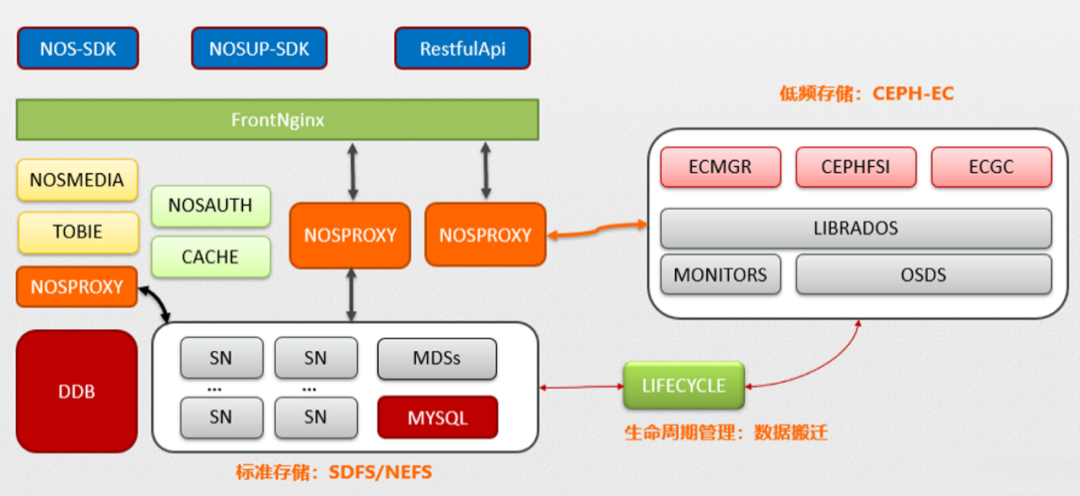
\includegraphics[width=0.9\textwidth]{NOS存储示意图.png}
    \caption{NOS存储示意图}
\end{figure}

\section{冗余恢复技术}%2.3
一台计算机是由若干个硬件组成的,随着技术的发展,这些硬件的故障率会控制的越来越低,但我们始终不能认为它们在工作期间都能正常运行。对于存储系统而言,最重要的则是存储介质,以磁盘为例,磁盘的年故障率大多可以保证低于1$\%$\cite{34},这在单机系统中几乎可以忽略不计,但是当磁盘的数量不断增加,系统中磁盘的总体故障率会大大增加。除了计算机内部的故障,存储系统还需要考虑外部环境的改变,例如断电断网等极端情况。因此,系统需具备一定的自动容错能力,通过存储冗余数据以防数据出现丢失,保证系统的可用性,多副本\cite{35}策略和纠删码\cite{36}是目前存储中常用的两种数据冗余方法。
\subsection{多副本}%2.3.1
系统通过多个副本来保存数据,一般副本个数为奇数个,当某个节点的数据丢失时,可以从副本中直接通过复制的方式进行恢复。这种方案的缺点是空间利用率较差,假设系统中为每份数据创建n-1份备份数据,那么实际的空间利用率仅为 1/n,占用了额外的空间,硬件的开销较大;这种方案的优点是数据备份比较容易,无需额外的计算,只需生成具有同样内容的副本即可,在写入时可以并行的写入,保证写入过程的高吞吐和稳定性,在策略恢复过程中也只需占用较少的网络负载。
\subsection{纠删码}%2.3.2
纠删码会将数据分成片段,将这些片段保存在不同的位置,当系统中某些片段的内容丢失或出现错误,可以通过其他正确的数据将丢失或有误的数据计算出来。这样做的代价是数据分段存储的时候需要进行计算,生成额外的校验数据后才能保证纠删码存储方式有效。

应用纠删码后,系统中的数据会写入数据块,生成的纠删码数据写入校验块,假设每份数据有k个数据块和m个校验块,当系统出现问题,有小于m个数据块中的数据不能正确读取,我们可以读取任意k个数据块,通过计算的方式将数据恢复。和多副本策略相比,纠删码策略无需保存整个副本,空间利用率较高,但是系统复杂,恢复数据和写入数据时需要进行读取和计算,会占用较多的CPU和内存,同时也会因为传输数据占用网络带宽,编码恢复率不及多副本策略。
\subsection{多副本和纠删码结合}%2.3.3
为了发挥以上两种冗余恢复技术的的优点,规避两者的缺点,人们想到可以将这两种策略同时使用,常见的方法有两种。一种是数据初始以多副本的形式写入多副本系统,经过一段时间,数据访问热度降低,再将数据批量地离线迁移到纠删码系统中;另一种是根据写入数据的大小来选择冗余存储的策略,小文件使用多副本来保存,占用的额外空间少,出现故障时也可以快速恢复,大文件用纠删码来保存,减少冗余副本的规模。

上述方案中的第一种需要批量迁移数据,迁移过程会带来额外的读写开销。本文采用基于条带的分配方式,将迁移的过程省略,提高系统整体性能。

\section{MongoDB}%2.4
MongoDB是一个广受欢迎的开源NoSQL数据库管理系统,它不像Mysql那样使用结构化的数据结构,而是采用了面向文档的数据模型,为应用程序提供了更加灵活的存储方案。以下是MongoDB的一些主要特点和功能:

1. 面向文档的数据模型

MongoDB使用JSON样式的BSON(二进制JSON)文档来存储数据。文档是一个动态结构的记录,可以容纳多种类型的数据,并且可以嵌套和索引。这种灵活性使得MongoDB适合处理各种类型和格式的数据。

2. 可扩展性和高性能

MongoDB支持水平扩展,应用需要扩展时可以轻松地增加实例节点进行横向扩展。同时它具有高效的读写操作和丰富的查询功能,可以处理大规模数据集和高并发访问。

3. 强大的查询语言

MongoDB提供丰富而灵活的查询功能,包括支持复杂条件、范围查询、正则表达式、地理位置查询等。它还支持聚合管道和全文搜索等高级查询操作,使开发人员能够快速、灵活地检索和分析数据。

4. 数据复制和故障恢复

MongoDB支持数据复制和故障恢复机制,通过复制集(replica set)实现数据的冗余存储和高可用性。

5. 自动分片

MongoDB支持数据的自动分片(sharding),将数据水平分割存储在多个分片服务器上。分片可以根据数据量和负载进行动态调整,以实现高效的数据存储和查询。

6. 多种语言和平台支持

MongoDB提供了丰富的驱动程序和客户端库,支持多种编程语言和开发平台。开发人员可以使用他们熟悉的语言和工具与MongoDB进行交互和集成。

7. 社区支持和活跃的生态系统

MongoDB拥有一个庞大的开源社区和活跃的生态系统,提供了大量的文档、教程、示例代码和第三方工具。这使得开发人员能够更好地学习和使用MongoDB,并从社区中获得支持和帮助。

由于MongoDB拥有优越的性能和灵活的数据模型,因此MongoDB被广泛应用于各种场景,包括Web应用程序、大数据分析、实时数据处理、物联网和日志存储等。其灵活性、可扩展性和强大的功能使得MongoDB成为当今流行的数据库解决方案之一。

MongoDB还提供了多种高可用性部署方式,以确保数据的可靠性和系统的持续可用性。以下是几种常见的高可用性部署方式:

1. 复制集(Replica Set)

复制集是MongoDB中最常用的高可用性部署方式。它由多个MongoDB实例组成,其中一个是主节点(Primary),负责处理写操作,其他节点是从节点(Secondary),负责处理读操作。如果主节点故障,MongoDB会通过选举从从节点中选出新的主节点。复制集提供了数据冗余、自动故障恢复和读取负载均衡的功能。

2. Sharding

使用MongoDB的Sharding模式可以很好地满足可用性和可扩展性,Sharding模式的架构如图2.6所示。

Sharding 模式下按照层次划分可以分为 3 个大模块:

(1)代理层:这是一个无状态的组件,起路由的作用。收到写请求的时候,代理层根据一定的规则决定数据的存储位置。收到读请求的时候,代理层要进行定位,根据写数据时应用的规则得出数据的访问地址,从而可以使客户端请求获取对应的数据。

(2)数据层:由一个个Replica Set集群组成,而Replica Set是由一个个存储节点组成,分为Primary节点和Secondary节点,在Primary节点不可用时会重新进行选举。

(3)配置中心:配置中心负责统一管理代理层和数据层,配置中心中会记录一些相关数据,比如Shard的数量、每个集群的节点组成、每个Shard里存储的数据量等。由于配置中心起到了元数据管理的作用,因此它和数据节点一样,有高可用的需求,所以在部署配置中心时,也采用了Replica Set的部署方式,保证数据的高可用。

\begin{figure}[h]
    \centering
    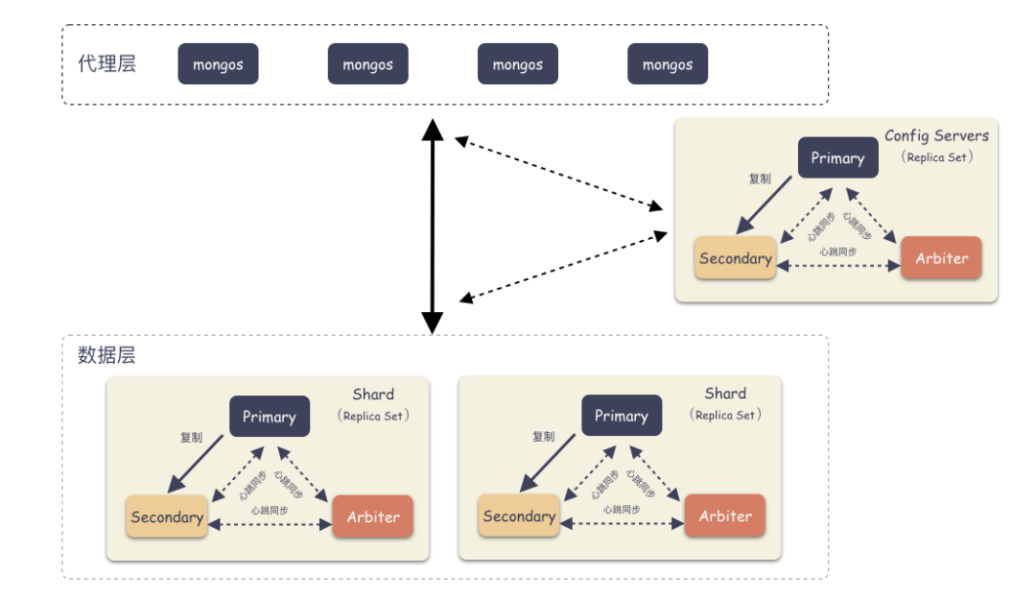
\includegraphics[width=0.95\textwidth]{MongoDB示意图.png}
    \caption{MongoDB的Sharding模式}
\end{figure}

3. 多数据中心部署

对于全球分布的应用程序,可以采用多数据中心部署来提供地理冗余和灾难恢复的能力。在这种部署方式中,MongoDB实例在不同的数据中心中进行部署,可以跨地理区域复制数据并配置故障转移策略,以确保数据的可用性和一致性。

通过高可用性部署方式可以保证MongoDB在运行过程中一直保持可用的状态,不会因为单点故障导致整个服务不可用,有效提升系统的稳定性。

\section{本章小结}%2.5
本章首先介绍了对象存储系统的体系结构,并分析了对象存储系统的优点。随后介绍了一些典型的分布式存储系统,本系统的实现多多少少被这些存储系统所影响。接下来介绍了存储系统中冗余恢复的技术,并分析不同方法之间的优缺点。最后介绍了MongoDB数据库,本论文实现的系统依赖MongoDB来保存一部分元数据。
